\setlength{\parskip}{\baselineskip}
\section{Results}

\begin{frame}
	\huge Results
\end{frame}

% Todo: Fill information
\begin{frame}{Compared Platforms: CPU}
	\center{\large{Some CPU model}}
	\begin{table}[H]
		\centering
		\begin{tabular}{ll}
			\toprule
			\textbf{Cores / Threads}      & x/x      \\
			\textbf{Max Turbo Frequency}  & x GHz   \\
			\textbf{TDP}                  & x W      \\
			\textbf{Max Memory Bandwidth} & x GB/s \\
			\textbf{Lithography}          & x nm     \\
			\bottomrule
		\end{tabular}
	\end{table}
\end{frame}

% Todo: Fill information
\begin{frame}{Compared Platforms: GPU}
	\center{\large{Some GPU model}}
	\begin{table}[H]
		\centering
		\begin{tabular}{ll}
			\toprule
			\textbf{CUDA Cores}        & x      \\
			\textbf{Tensor Cores}      & x        \\
			\textbf{GPU Memory}        & x GB GDDR6 \\
			\textbf{Boost Clock}       & x MHz  \\
			\textbf{Memory Interface}  & x-bit   \\
			\textbf{Memory Bandwidth}  & x GB/s   \\
			\textbf{Power Consumption} & x W      \\
			\bottomrule
		\end{tabular}
	\end{table}
\end{frame}

% Todo: Fill information
\begin{frame}{Compared Platforms: FPGA}
	\center{\large{Some FPGA Platform}}
	\begin{table}[H]
		\centering
		\begin{tabular}{ll}
			\toprule
			\textbf{PL/DSP Clock Frequency} & x/x MHz \\
			\textbf{LUT Usage}              & x\%      \\
			% 		\textbf{LUTRAM Usage} & -\\
			\textbf{FF Usage}               & x\%     \\
			\textbf{BRAM Usage}             & x\%     \\
			\textbf{DSP Usage}              & x\%     \\
			% 		\textbf{BUFG Usage} & -\\
			\bottomrule
		\end{tabular}
	\end{table}
\end{frame}

% Todo: Fill information
\begin{frame}{Compared Platforms: FPGA}
	\center{\large{Proposed Platform}}
	\begin{table}[H]
		\centering
		\begin{tabular}{ll}
			\toprule
			\textbf{Clock Frequency (MHz)} & xMHz \\
			\textbf{LUT Usage}             & x\% \\
			\textbf{LUTRAM Usage}          & x\% \\
			\textbf{FF Usage}              & x\% \\
			\textbf{BRAM Usage}            & x\% \\
			\textbf{DSP Usage}             & x\%  \\
			% \textbf{BUFG (\%)}             & x\% \\
			\bottomrule
		\end{tabular}
	\end{table}
\end{frame}

% Todo: Fill configuration information
\begin{frame}{CPU \& GPU Performance}
	\begin{itemize}
		\item Config 1
		\item Config 2
		\item Config 3
	\end{itemize}
\end{frame}

% Todo: Replace graph
\begin{frame}{CPU \& GPU Performance: Latency}
	\centering
	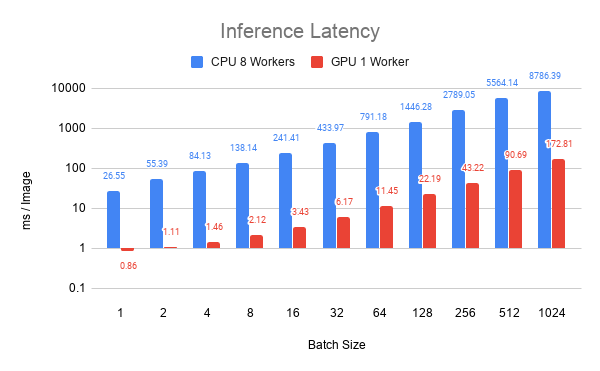
\includegraphics[width=0.7\textwidth]{../Images/Results/CPU-GPU-Inference-Latency.png}\\
\end{frame}

% Todo: Replace graph
\begin{frame}{CPU \& GPU Performance: Throughput}
	\centering
	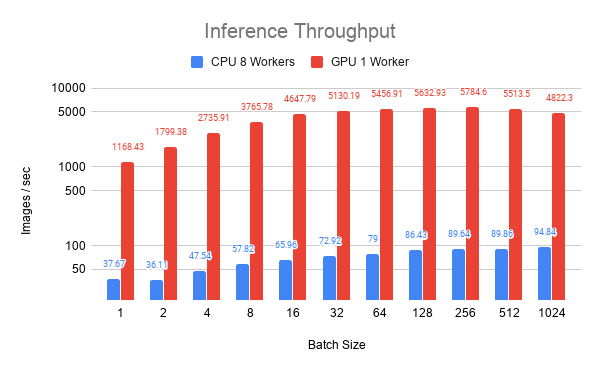
\includegraphics[width=0.7\textwidth]{../Images/Results/CPU-GPU-Inference-Throughput.png}\\
\end{frame}

% Todo: Fill information
\begin{frame}{Final Performance}
	\begin{table}[H]
		\centering
		\begin{tabular}{l|l|l|l|l}
			\toprule
			                                    & \textbf{CPU} & \textbf{GPU} & \textbf{CHaiDNN} & \textbf{Proposed Platform} \\
			\midrule
			\textbf{Clock Frequency (MHz)}      & x				& x				& x					& x							\\
			\textbf{Throughput (Images/s)}      & x				& x				& x					& x							\\
			\textbf{Throughput Speedup}         & 100\%			& x\%			& x\%				& x\%						\\
			\textbf{Latency (s)}                & x				& x				& x					& x							\\
			\textbf{Latency Speedup}            & 100\%			& x\%			& x\%				& x\%						\\
			\textbf{Total On-Chip Power (Watt)} & x				& x				& x					& x							\\
			\textbf{Power Efficiency}           & 100\%			& x\%			& x\%				& x\%						\\
			\textbf{Energy Cons./Image (Joule)} & x				& x				& x					& x							\\
			\textbf{Energy Efficiency}          & 100\%			& x\%			& x\%				& x\%						\\
			\textbf{Images/Joule}               & x				& x				& x					& x							\\
			\bottomrule
		\end{tabular}
	\end{table}
\end{frame}

% Todo: Replace graph
\begin{frame}{Final Performance}
	\centering
	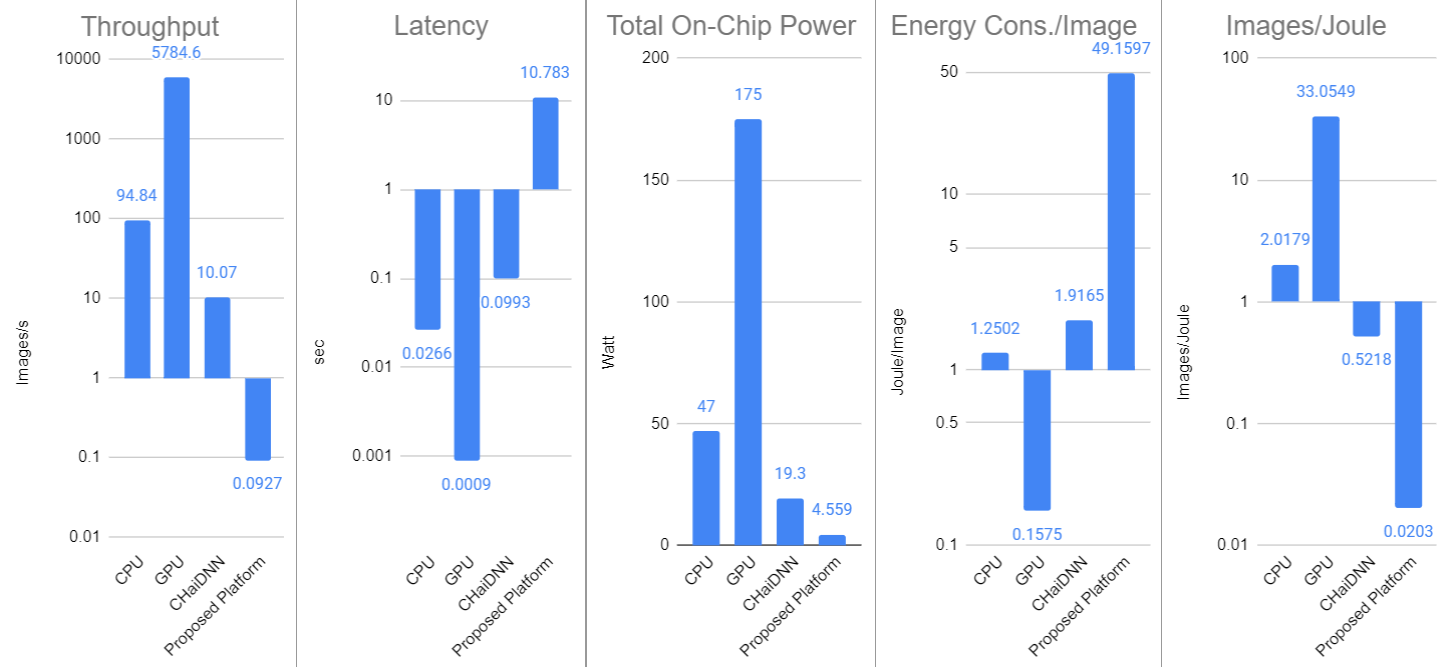
\includegraphics[width=0.9\textwidth]{../Images/Results/Final-Results-charts.png}\\
\end{frame}
